\section{Design patterns}

\subsection{UML}

\subsubsection{Classes}

\begin{figure}[h]
\caption{UML arrows}
\centering
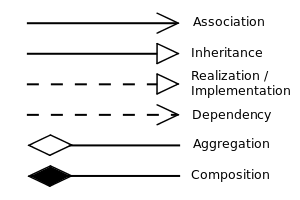
\includegraphics[width=0.4\textwidth]{images/umlArrows.png}
\end{figure}


\begin{figure}[h]
\caption{UML classes}
\centering
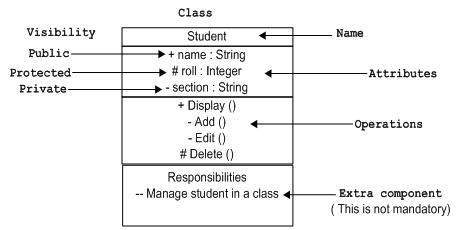
\includegraphics[width=0.8\textwidth]{images/umlClass.jpg}
\end{figure}

\subsubsection{Sequences}

\subsubsection{Usecases}

\subsection{Dependencies versus microservices}

Dependencies can be included right in your sourcode. Microservices on the other hand are not included at all, but called remotely from your programm. 


\begin{table}[h]
\centering
\caption{Dependencies versus microservices}
\begin{tabular}{@{}lllll@{}}
\toprule
        & Dependencies                                             & Microservices                                                      &  &  \\ \midrule
Changes & You can include the exact needed version of a dependency & Your program needs to adapt immediately if the service API changes &  &  \\
        &                                                          &                                                                    &  &  \\
        &                                                          &                                                                    &  &  \\ \bottomrule
\end{tabular}
\end{table}


\subsection{Strategy pattern}

The strategy pattern (also known as the policy pattern) is a behavioral software design pattern that enables selecting an algorithm at runtime. Instead of implementing a single algorithm directly, code receives run-time instructions as to which in a family of algorithms to use.[1]

Strategy lets the algorithm vary independently from clients that use it.[2] Strategy is one of the patterns included in the influential book Design Patterns by Gamma et al.[3] that popularized the concept of using design patterns to describe how to design flexible and reusable object-oriented software. Deferring the decision about which algorithm to use until runtime allows the calling code to be more flexible and reusable.

For instance, a class that performs validation on incoming data may use the strategy pattern to select a validation algorithm depending on the type of data, the source of the data, user choice, or other discriminating factors. These factors are not known until run-time and may require radically different validation to be performed. The validation algorithms (strategies), encapsulated separately from the validating object, may be used by other validating objects in different areas of the system (or even different systems) without code duplication.

\begin{figure}[h]
\caption{Strategy design pattern}
\centering
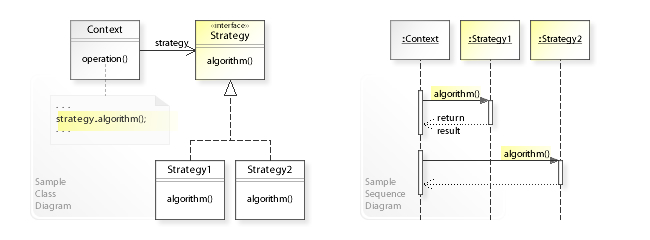
\includegraphics[width=0.95\textwidth]{images/strategyDesignPattern.jpg}
\end{figure}

\subsection{State pattern}

The state pattern is a behavioral software design pattern that allows an object to alter its behavior when its internal state changes. This pattern is close to the concept of finite-state machines. The state pattern can be interpreted as a strategy pattern, which is able to switch a strategy through invocations of methods defined in the pattern's interface.

The state pattern is used in computer programming to encapsulate varying behavior for the same object, based on its internal state. This can be a cleaner way for an object to change its behavior at runtime without resorting to conditional statements and thus improve maintainability.

The state pattern is set to solve two main problems:
\begin{itemize}
        \item An object should change its behavior when its internal state changes.
        \item State-specific behavior should be defined independently. That is, adding new states should not affect the behavior of existing states.
\end{itemize}

\begin{figure}[h]
\caption{State design pattern}
\centering
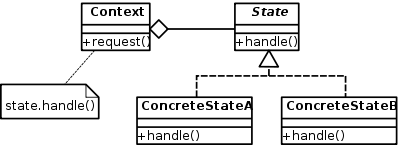
\includegraphics[width=0.95\textwidth]{images/stateDesignPattern.png}
\end{figure}

\subsection{Observer pattern}

The Observer pattern addresses the following problems:
\begin{itemize}
        \item A one-to-many dependency between objects should be defined without making the objects tightly coupled.
        \item It should be ensured that when one object changes state an open-ended number of dependent objects are updated automatically.
        \item It should be possible that one object can notify an open-ended number of other objects.
\end{itemize}

\begin{figure}[h]
\caption{Observer design pattern}
\centering
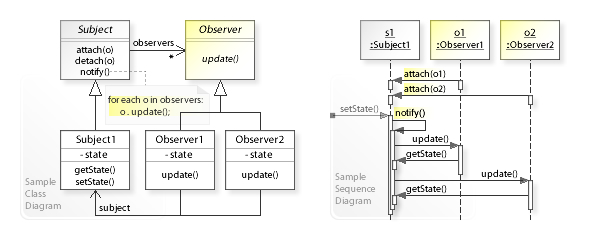
\includegraphics[width=0.95\textwidth]{images/observerDesignPattern.jpg}
\end{figure}


\subsection{Orchestration: Workflow pattern}

\subsection{Choreography: Actor pattern}

\subsection{Monads}

\subsubsection{Maybe-monad}

Maybe-monads make sense when a function might return null, which we want to avoid. A user can only access the value after he has specified what shoud happen if the value is null. In its simplest form, this could be done like this: 
A nice implementation can be found \href{https://codewithstyle.info/advanced-functional-programming-in-typescript-maybe-monad/}{here}.

\begin{lstlisting}[language=java]
class Maybe<T> { 
    private value: T | null = null;

    constructor(val: T | null) {
        this.value = val;
    }

    public getVal(ifNull: T): T { 
        if (this.value) return this.value;
        else return ifNull;
    }
}

// a function that might return null
function divide(dividend: number, divisor: number): Maybe<number> { 
    return new Maybe<number>(dividend / divisor);
}

// we can only get the result of the calculation after specifying what should happen if null is returned. 
function divideAndResolve(dividend: number, divisor: number, deflt: number): number { 
    let maybeResult = divide(dividend, divisor);
    return maybeResult.getVal(deflt);
}

console.log("10/2 = ...", divideAndResolve(10, 2, 0));
console.log("10/0 = ...", divideAndResolve(10, 0, 0));
\end{lstlisting}